% For tracking purposes - this is V3.1SP - APRIL 2009

\documentclass{acm_proc_article-sp}

\usepackage{graphicx}
\usepackage{alltt}
\renewcommand{\ttdefault}{txtt}

\begin{document}

\title{Attribute Learning System}
\subtitle{[Applying Genetic Algorithms to Improve RPG Combat Mechanics]} % Dude that title sucks


\numberofauthors{2} 

\author{
% 1st. author
\alignauthor
Austin Cory Bart\\
       \affaddr{Virginia Tech}\\
       \email{acbart@vt.edu}
% 2nd. author
\alignauthor
K. Alnajar\\
       \affaddr{Virginia Tech}\\
       \email{kar@vt.edu}
\alignauthor
}

\date{24 April 2013}

\maketitle
\begin{abstract}
Having a good set of moves for players to choose from in role-playing games (RPG) is essential for the game to succeed.  Often times in an RPG, the players have various attributes which these moves can effect and coming up with good formulas for this is not easy. The process of creating an effective set of moves can take time and can be a difficult challenge to overcome in the design process. This paper propeses an implementation to effectively create these moves using a genetic algorithm implementation. Two seperate implementation styles of genetic algorithms are used, a tree style and a vector style. The results show that the vector styled approach for the genetic algorithm shows promising results in move set creation.
\end{abstract}

% A category with the (minimum) three required fields
% TODO: We need to look up the tags for this research area
\category{1.2.1}{ARTIFICIAL INTELLIGENCE}{Applications and Expert Systems --- \textit{games}}

\terms{Genetic Programming}

\keywords{Genetic, Programming, Game, Development} % NOT required for Proceedings

\section{Problem}

In the design of role-playing games (RPGs), one of the most challenging aspects is finding a functional set of moves that players can utilize against opponents and other players. The challenge is that moves should take advantage of the design of the system created, while being enjoyable to use and not overly complicated. At the same, the moves should be just complicated enough that players will need to have a good understanding of the game and their own capabilities in order to become effective players. Creating a set of moves that fall within this criteria can be a time consuming task for game developers, as large move sets will need to be thought up and tested. There is a vast number of forms that moves could take on, even in a system with a small number of attributes.
The goal in designing this system was to assist in the development of RPG style games, or any games in which a distinct set of moves can be used on an opponent. The system is geared towards game developers, with the intention that by manipulating the configuration of the system, it will assist in producing unique movesets with some level of strategic play integrated.
In the context of this system design, we define attributes as a set of descriptors of the state of a player in the game. For example, health, attack, and defense may be a player’s attributes. A primary attribute is one which is important in determining the outcome of a player battle, such as determining a player to have lost if that player’s primary attribute, health, reaches zero. A move as an action taken by a player that may modify that player’s own attributes or the opponent’s attributes. A movelist is the list of moves available to a player. In a simulated battle, the players take turns using moves to affect each others’ attributes, with the objective being to minimize the primary attributes of the opponent player and “win” the battle.

\section{Approach}

\subsection{Prior Work}

When looking at the literature associated with this problem, it seemed that this was an interesting and unique problem that did not have substantial solutions directly focused on solving this challenge. Closely related, Zook and Riedl (2012) examine dynamic difficulty adjusment for players with varying degrees of game skill. Their paper focuses on challenge tailoring in a role-playing style game using a temporal player model to assist in predicting future strength. This concept proposes a way for games to self monitor and adapt based on player action. This [NOT DONE AT ALL]

Dynamic Difficulty Adjustment

\subsection{Approach}

Because the state space is extremely large with many local maxima, we used a genetic algorithm. A genetic algorithm mimics the natural process of evolution by repeatedly manipulating a population of \textit{phenotypes}. These phenotypes are composed of mutable properties called \textit{genes}. Each new iteration of a population is called a \textit{generation}. A phenotype can be changed via mutation - where properties are changed at random - and via cross-over - where properties are combined with the properties of another phenotype. A \textit{fitness function} maps the phenotypes to a real number that indicates that phenotype’s value. 
We performed a number of experiments with our genetic algorithm in order to develop balanced moves. In particular, we investigated the effect that varying parameters had on our rate of utility growth and maximal utility achieved. As we gathered data, we did additional experiments to evaluate the validity of the results achieved.

\section{Implementation of the Genetic Algorithm}

In our system, the phenotype is a Movelist, a union of two sets of moves (one set for each player). A move is abstractly defined as a function that maps a set of input attributes to a single output attribute. While designing our system, we explored two different implementations of moves. Additionally, we experimented with a number of fitness functions.

\subsection{Fitness Function}

We based our fitness function on the results of battle simulations between two players.  The two player types used were based on Minimax algorithms with a depth limit of four. Each player was given a moveset from which to select in their action state. The utility of the selected moves in the Minimax algorithm were based on maximizing the primary attributes of each player.
Once a single battle simulation completes, we use various statistics from the simulation to calculate the fitness. A number of approaches were taken in determining the overall fitness for a set of moves:

\begin{description}
    \item[Move Usage] In an ideally balanced game, all moves should be used approximately equally. Over the course of a battle, we keep track of all the moves used as a ratio of the total moves used. Then, the standard deviation of these percentages is calculated. A well balanced game - where moves are used evenly - has a low standard deviation, but an unbalanced game will have a high deviation.
    \item[Battle Victory] In a typical game, there should be final victory or outcome between the players. This metric awarded a positive utility for battles that involved a victor and a negative reward for battles that ended in a stalemate.
    \item[Battle length] We believed that a good game should last with in a certain range of turns. This way the battles are neither too short (where one player has an overt advantage) or too long (where neither player is able to gain an advantage). 
    \item[Linearity] In order for a battle to progress smoothly in an ideal battle, each player should show a steady decrease in primary attributes, rather than a sudden loss at a single point in the battle. This function looked at the progression of player statistics and gave a high utility for battles where both the players’ progress was a steady decrease in attributes, and a negative utility for sudden or extreme changes in the player attributes.
\end{description}

Preliminary testing revealed the most success with a fitness function based on Move Usage and Battle Victory. After analyzing the results from the Linearity metric, we determined that this led to battles where the secondary attributes were underrepresented, which was antithesis to our goals. Since we desired consistency in our utility function across all results, during our experiments we did not include Battle Length and Linearity in our calculations.

\subsection{Move}

As previously mentioned, our system defines a Move as an abstract function to map one state of the battle to the next. A state in the battle can be seen as a vector of the two players’ attributes, demonstrated in \ref{example move transformation}. 

\subsection{Function Tree}

We first attempted to represent moves as Abstract Syntax Trees of operators over attributes. Every node in the AST is an \textit{operator}, with zero-arity operators (which yield attributes from the input vector, unmodified) being terminal nodes. Early experiments with \textit{ephemeral nodes} - coded as zero-arity operators that returned a constant value, as opposed to an attribute - led to their inclusion. \ref{example function tree} gives an example of a Function Tree with a binary operator (addition), unary operator (doubling), and two nullary operators (an attribute and an ephemeral constant).

\subsubsection{Mutation Algorithm}

There are many well-known methods for mutating an AST, so we chose to implement an interesting subset of them. 
\begin{description}
    \item[Subtree Mutation] A subtree is selected, and is given a new parent. This new, taller subtree replaces the original, increasing the depth of the tree.\cite{geneticprogramming.us}
    \item[Node Replacement Mutation] A node is selected and replaced
\end{description}
    Preliminary tests of the mutation algorithms revealed that they had an undesirably dramatic effect on the structure of the Function Tree. \ref{Entire Tree Mutation Amount vs. Edit Distance} demonstrates how repeatedly mutating the entire tree has almost random impact on the Levenshtein Edit Distance between the mutant and the original. In order to keep mutational changes to a minimum, we refactored the algorithms to only affect terminal and pre-terminal nodes. The result of this change is demonstrated in \ref{Terminal Mutation Amount vs. Edit Distance}, which shows a logarithmic relationship between the number of times a tree is mutated and the Edit Distance from its parent.
    
    \subsubsection{Cross-over Algorithm}
    
The problem of crossing over Abstract Syntax Trees is well-established in the literature. We investigated several possible implementations before choosing one based on work by Poli and Langdon \cite{crossover}. Their uniform cross-over algorithm matches common nodes in the two parents trees, starting from the root. When dissimilar parallel nodes (named \textit{Boundary Nodes}) are encountered, a subtree is chosen randomly from the two options. 

Unfortunately, although this implementation was described favorably in the literature, we found that it rarely caused a true combination of the parents, but instead led to one parent being copied wholesale in favor of the other. \ref{cross-over similarity} graphs the result of a 1000 trials where two parents were randomly generated and then crossed with each other. The Percentage Difference from Parent was calculated as the change in edit distance from one parent to the child over the edit distance of the two parents. Ideally, this distributed would be heavily banded around 50%; instead, more than 3/5 of the data is at 0% or 100% percent difference (indicating a parent was copied completely).
    
    \subsubsection{Validation of Trees}
    
Although we performed structural analysis of the our Function Tree implementation, we were doubtful that these structural modifications would have a corresponding impact on the numerical results of the functions. For example, changing a function of the form “player 1’s 1st primary attribute + player 2’s 1st secondary attribute” to use division instead of addition would yield a largely different set of outputs. In order to quantitatively measure the similarity of two functions, we used a two-sample Kolmogorov–Smirnov test. This variant of the KS-test is a non-parametric method for determining if two sets of samples come from the same distribution. 
Because the KS-test expects one-dimensional data, the domain of the inputs (normally multivariate) was restricted from the real numbers to [-100,100], and their cross-product treated as a single input. For example, in a system with one primary attribute and one secondary, the Function Tree would have $$|(100) - (-100)|^4 = 1600000000$$ integer inputs and outputs, following the form $$<-100, -100, -100, -100> , <-100, -100, -100, -99>$$
$$ ... $$
$$<99, 100, 100, 100> , <100, 100, 100, 100>$$ 

To calculate our samples, we strode over the inputs at a moderate pace in order to further reduce the domain. A value of 1 from the test indicates evidence of two completely different functions, whereas a value of 0 indicates evidence of two identical functions.
In our validation trials, we generated two trees randomly, measured their edit distance, and then graphed that metric against the results of a KS-test. \ref{edit distance to ks-test for trees} shows the surprisingly strong correlation between Edit Distance and the KS-Test. Unfortunately, it also demonstrates a weakness of the Function Tree implementation: the values quickly get very high (reaching .4), which means that we expand through the search space extremely quickly even when performing a single mutation.

	\subsection{Function Vector}
    
Function Trees suffer from a lack of fine state exploration. A single mutation can cause relatively drastic changes to the function. For this reason, we decided to implement and compare an alternative model - functions described as vectors, dubbed Function Vectors.

The function vectors were modeled as vectors of coefficients. In this model, each attribute was assigned a coefficient. In addition, the vector had a constant that could be used for additional adjustments to the vector equation. Due to the fundamental difference between the vector and tree scheme a different approach was taken for the mutation and cross-over algorithms. 
    
    \subsubsection{Mutation Algorithm}
    The mutation of the vector functions was performed using a randomly generated coefficient within a specified range. This allowed for manipulation of the vectors in a significantly reduced space. This was verified in a [KS-test] validation, which showed that the mutations acting upon the vectors had a subtle influence.
    
    \subsubsection{Cross-over Algorithm}
    The cross-over algorithm of the vector functions utilized the coefficients to find an average between coefficients of similar attribute effectors within the vector equations. Testing showed this to be significantly effective in producing new moves with high utility.
    
    \subsubsection{Validation of Vectors}
    To validate the vector mutation function we used the Kolmogorov-Smirnov (K-S)  test to look at the difference in changes made by mutation. The results of the K-S test showed only a marginal amount of change (R2=0.14), which was expected given the limitation imposed on the range of possible coefficients allowed.
    Validation of the cross-over function for vectors was done through comparison and analysis of initial battle simulations and iterations. Looking at the utility results when running initial tests showed a correlation between a high cross-over rate and improved utility.
    
    
    \section{Experiments}

\begin{figure*}[ht!]
\centering
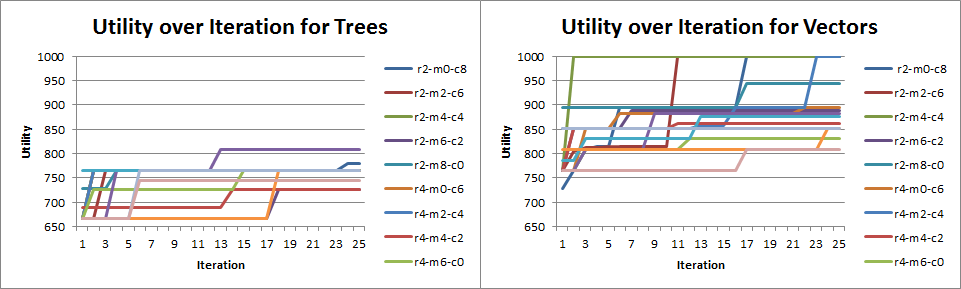
\includegraphics[width=\textwidth,height=90mm,keepaspectratio]{./images/gen-mureco-comparison.png}
\caption{A simple caption}
\label{utility_experiments}
\end{figure*}
    
    \subsection{Move Generation Experiments}

In order to collect data on the effectiveness of the system and validate the moves, 25 iterations were run over a variety of conditions. The base conditions of the algorithm were set as follows, unless manipulated for the purpose of a particular experiment: a constant population of 500 movesets, both players were Minimax players with a look-ahead depth of four, mutation was set to 50%, cross-over was set to 20%, the parent retention was set to 30%, and the attributes frequency was set to one primary and two secondaries.    

    \subsubsection{Tree vs. Vector}

Both the tree and vector implementations were tested evenly in the experiments under the various conditions. The results of the highest utilities of each type of implementation across the iterations can be seen in the graph. The vector implementation significantly outperformed the tree implementation across nearly every experiment, with the highest tree utility failing to break a value of 825-utility, whereas the vector implementation reached a 1000-utility score multiple times across various experiments. 

    \subsubsection{Mutation Rate vs. Cross-over Rate vs. Parents Retained}

To see the effects of various conditions on the genetic algorithm, these variables were manipulated in multiple experiments, and the effects of these changes can be seen in the utility over iteration graphs. The results show that for the tree implementation, an equal 20% retention and cross-over rate, with a 40% mutation rate yielded the best results. For the vector implementation, experiments with a high percentage allocated to the mutation and cross-over conditions showed the greatest utility output. The most effective of the conditions was when the mutation and cross-over were equal, with the condition set to 20% retention, 40% mutation and 40% cross-over. This showed a high starting utility and had a moveset with a utility of 1000 after the first iteration.

    \subsubsection{Attribute Type Frequencies}

\begin{figure*}[ht!]
\centering
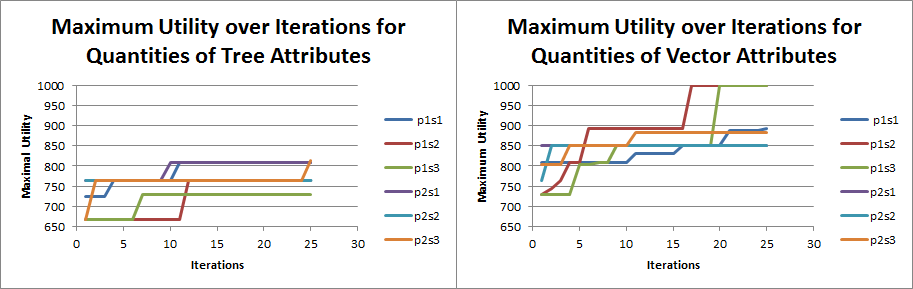
\includegraphics[width=\textwidth,height=90mm,keepaspectratio]{./images/attr_frquency_comparison.png}
\caption{A simple caption}
\label{attribute_frequency_experiments}
\end{figure*}

In these tests, we wanted to look at what effect the number of primary and secondary attributes may have on the overall utility of movesets. To this, attribute type frequencies were tested with combinations of 1 to 2 primary attributes and 1 to 3 secondary attributes. Results of these tests can be seen in the given graphs [graph reference]. For the tree implementation, the tests vary little effect on the outcome utilities, with the average consistently ranging in the 750 utility range. The results of the vector tests showed a greater effect of attribute frequency on the utility. The utility of tests conducted with a single primary attribute were yielded a higher maximum utility, with a 1000 utility reached in the tests with a single primary attribute, and either two or three secondary attributes. This testing validated the use of the default single primary attribute with two secondary attributes that was used for the attribute type frequencies in the other experiments.
    
    \subsection{Validation of Moves}

To look at the effectiveness of the moves generated by our solution, we chose to validate the movesets by using a strategic Minimax player, and a nonstrategic (random) or lower level Minimax player to simulate a battle with the moves. If the moves produced were viable, then the expected outcome of this testing would show that a strategic player would outperform and defeat a random or lower level player.
The results of this testing did not show what was expected. In many battle simulations the lower level Minimax was able to defeat the higher level Minimax player, and in some cases the random player was able to defeat the Minimax player. After looking at the movesets on a case by case basis, it was found that the test results which did not follow the prediction was due to an issue in the way moves that affected the primary status of the opponent had been formed. In these cases. the losing player often had no move that would be able to reduce a primary attribute of the other player in order to win.
    
    \section{Conclusion}

The overall results of our move validation experiments showed that the movesets were not applicable in a true RPG setting. The poor results of the validation is most likely due to the utility function that determines the value of the movesets not properly taking into account an equal chance for each player to win the match through strategy.  It became apparent that the utility function used for the movesets did not take into account a practical usage of the moves to defeat the opponent in all circumstances. The failure to take this feature of battles into account meant that though the move usage was strategic and distributed evenly, and there was a victor associated, it provided no opportunity for the player with the moveset that lacked a strong primary reducing move to win the battle. This makes the movesets generated by the system unusable in a practical application.
	However, we did find that in cases where both players were given a set of moves where each had an effective primary reducing move, the results of the validation experiments were 

	%FINISH THIS SECTION
    
    %We need to do work!
    
    \section{Future Work}

As indicated by the results of our failed validity tests on the movesets, the most immediate work that needs to be done is a redesign of the utility function calculation. It is possible that given a utility function that takes into account overlooked aspects of the usage in these simulations, movesets which may be applied more practically in a game design could be generated by the system.
	It would be interesting to look at abstracting the design of the individual moves to provide flexibility for other game engines. In our original design, we proposed a system where every move has a unique function behind it. However, some games use a single formula for every move, and then assign unique attributes on a per-move basis (such as “Base power” or “Accuracy”, in addition to player attributes. Supporting game engines such as these might dramatically alter the search space, but could lead to more tenable results.
	Finally, we will explore a trending alternative to traditional genetic algorithms called \textit{Novelty Search}. The Novelty Search algorithm rewards new behavioral changes in a phenotype, rather than applying a fitness function. By removing the focus on moving towards an objective, which can make it difficult to break out of deceptive local maxima, this algorithm has been shown to be effective for certain problem domains. Given this still inchoate research problem, applying Novelty Search or another variant search algorithm could be a fruitful strategy.
    
    


%
% The following two commands are all you need in the
% initial runs of your .tex file to
% produce the bibliography for the citations in your paper.
\bibliographystyle{abbrv}
\bibliography{sigproc}  % sigproc.bib is the name of the Bibliography in this case
% You must have a proper ".bib" file
%  and remember to run:
% latex bibtex latex latex
% to resolve all references

\begin{thebibliography}{1}

% Bibliography goes here

\end{thebibliography}

%Generated by bibtex from your ~.bib file.  Run latex,
%then bibtex, then latex twice (to resolve references)
%to create the ~.bbl file.  Insert that ~.bbl file into
%the .tex source file and comment out
%the command \texttt{{\char'134}thebibliography}.

\balancecolumns
% That's all folks!
\end{document}
